\documentclass[11pt,a4paper]{article}
\usepackage[T1]{fontenc}
\usepackage[utf8]{inputenc}
\usepackage{lmodern}
\usepackage[spanish,es-tabla]{babel}
\usepackage[a4paper,margin=2.4cm]{geometry}
\usepackage{booktabs,graphicx}
\usepackage[hidelinks]{hyperref}

\setlength{\parindent}{0pt}
\setlength{\parskip}{0.5em}
\urlstyle{same}
\raggedbottom

\begin{document}
\begin{center}
{\LARGE Fotovoltaica visible en Cantabria\par}
\smallskip
{\large Resultados y aplicaciones\par}
\medskip
{\small Noviembre de 2026}
\end{center}

El panel de indicadores muestra \textbf{27,28 ha de paneles detectados} en toda la zona procesada en 2023. El análisis energético de este informe usa el \textbf{inventario de seguimiento}, que reúne \textbf{15,21 ha de detecciones de 2023} en emplazamientos seleccionados para revisar su evolución. Ambas cifras son superficies vistas desde arriba.

\section{Distribución territorial en 2023}

La pasada regional procesó 957\,468 teselas y produjo 18\,868 componentes de segmentación. El recuento se refiere a conjuntos de píxeles y una misma instalación puede estar dividida en varios componentes. Santander (3,02 ha), Medio Cudeyo (2,61 ha), Camargo (1,97 ha) y El Astillero (1,70 ha) concentran juntos el \textbf{34,1\,\% del área detectada}. El mapa representa superficie absoluta por municipio.

\begin{figure}[!ht]
\centering
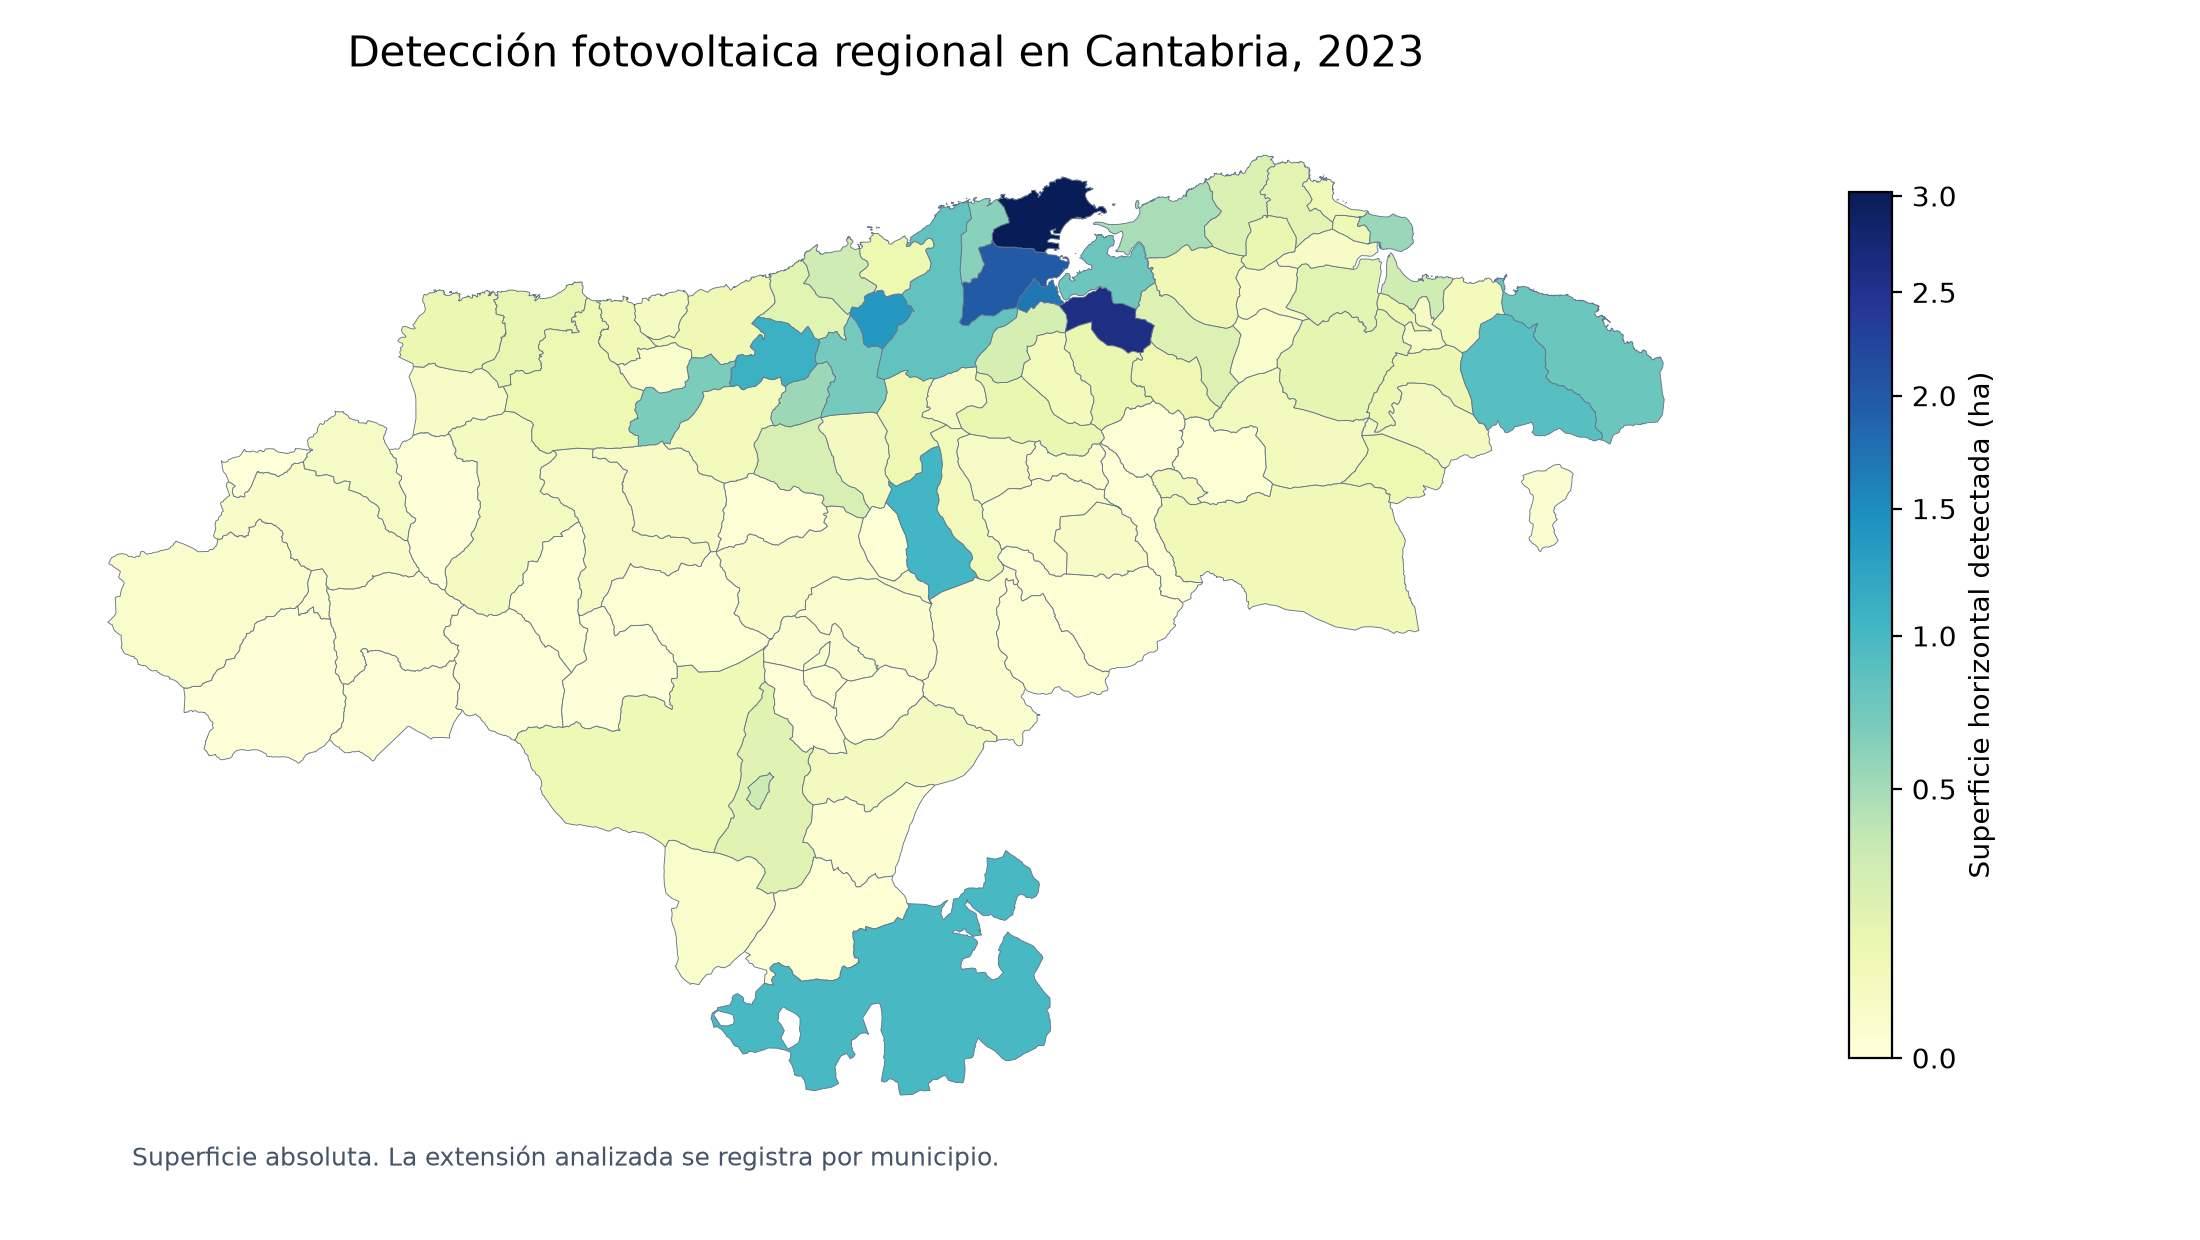
\includegraphics[width=0.98\linewidth]{figuras/mapa_deteccion_regional_2023.png}
\caption{Superficie detectada en la pasada regional, agregada por municipio. Elaboración propia con ortofotos PNOA de 2023 y límites municipales.}
\label{fig:regional}
\end{figure}

El cruce con la cartografía de edificios sitúa 21,16 ha (77,6\,\%) dentro de sus huellas y 6,13 ha (22,4\,\%) fuera. Un filtro que solo conserve píxeles dentro de las huellas elimina casi una cuarta parte de la superficie detectada. La categoría exterior describe el resultado del cruce cartográfico. La revisión visual permite distinguir los paneles sobre el terreno de detecciones desplazadas o cubiertas ausentes en la capa de edificios.

En la evaluación local de 988 teselas, el detector recuperó el 82,4\,\% de los píxeles de panel anotados y el 89,1\,\% de los píxeles detectados coincidió con las etiquetas. Las métricas corresponden al test local de 2023. La memoria técnica documenta el protocolo de evaluación.

\clearpage

\section{El inventario de seguimiento}

Para 2023, el seguimiento recupera los contornos automáticos de los emplazamientos que se marcaron como presentes en la revisión. Ese conjunto suma 15,21 ha horizontales. Para consultar las fichas históricas en el panel, selecciona una campaña anterior o la muestra comparable. El mapa de la campaña de 2023 permite explorar la detección regional por municipio.

Una ficha reúne los grupos de paneles atribuidos al mismo edificio o vinculados por su coincidencia espacial entre vuelos. Sirve para seguir un emplazamiento y sumar la superficie de sus paneles sin duplicar solapes. La ficha es una agrupación cartográfica provisional. La columna de estado distingue la presencia observada, la ausencia revisada y los casos sin evidencia suficiente.

\begin{figure}[!ht]
\centering
\begin{minipage}[t]{0.485\linewidth}
\centering\small\textbf{2020 · anotación manual}\\[2pt]
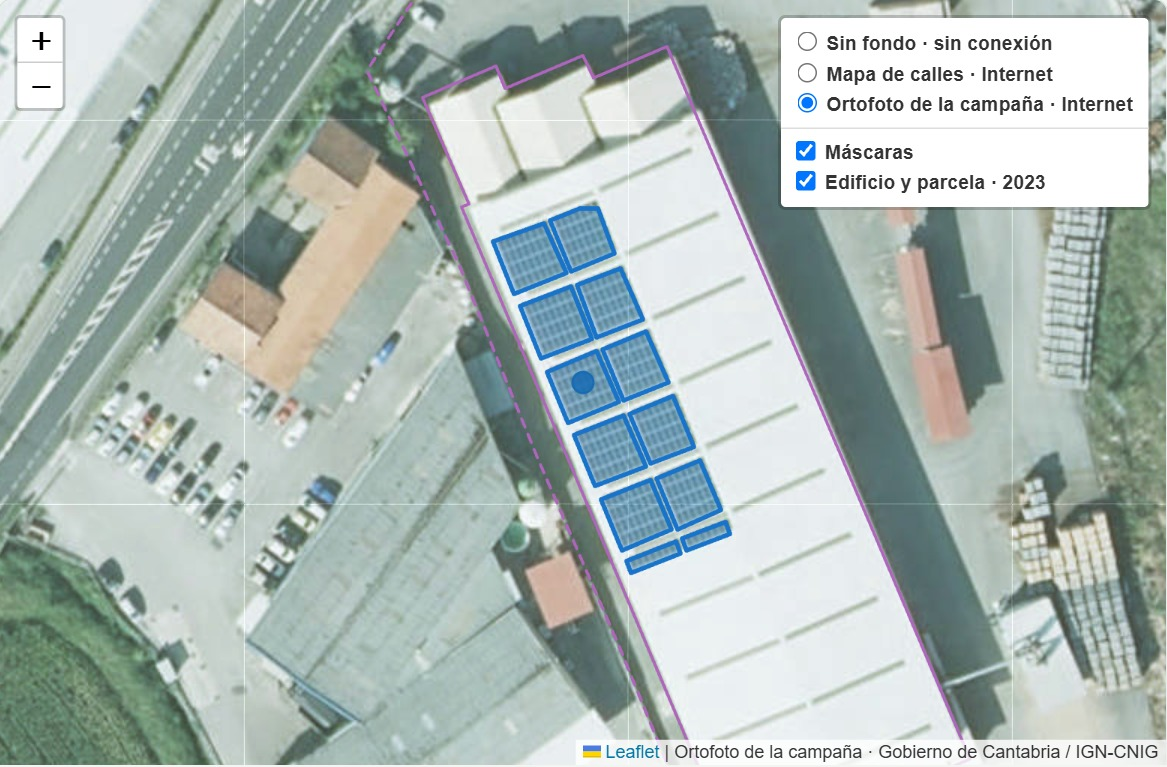
\includegraphics[width=\linewidth]{figuras/panel_pielagos_2020.jpg}
\end{minipage}\hfill
\begin{minipage}[t]{0.485\linewidth}
\centering\small\textbf{2023 · detección automática}\\[2pt]
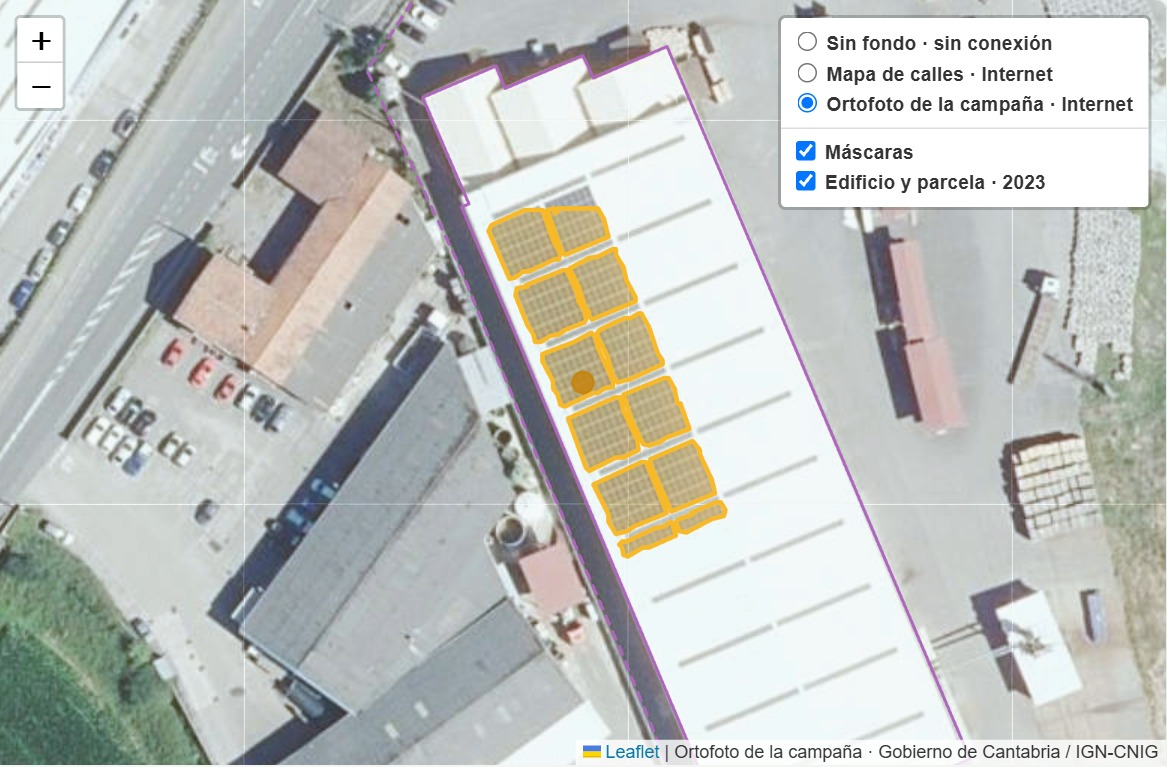
\includegraphics[width=\linewidth]{figuras/panel_pielagos_2023.jpg}
\end{minipage}
\caption{Nave de Piélagos en el inventario de seguimiento. Azul, anotación manual. Ámbar, máscara automática. Violeta, edificio y parcela de referencia. Ortofotos del Gobierno de Cantabria e IGN/CNIG.}
\label{fig:pielagos}
\end{figure}

La ficha de la figura~\ref{fig:pielagos} reúne los bloques de paneles de una misma nave. Recoge 614,1 m\textsuperscript{2} anotados en 2020 y 629,3 m\textsuperscript{2} detectados en 2023. La ortofoto y los contornos dejan a la vista qué zonas del tejado se incluyeron en el cálculo.

\begin{figure}[!ht]
\centering
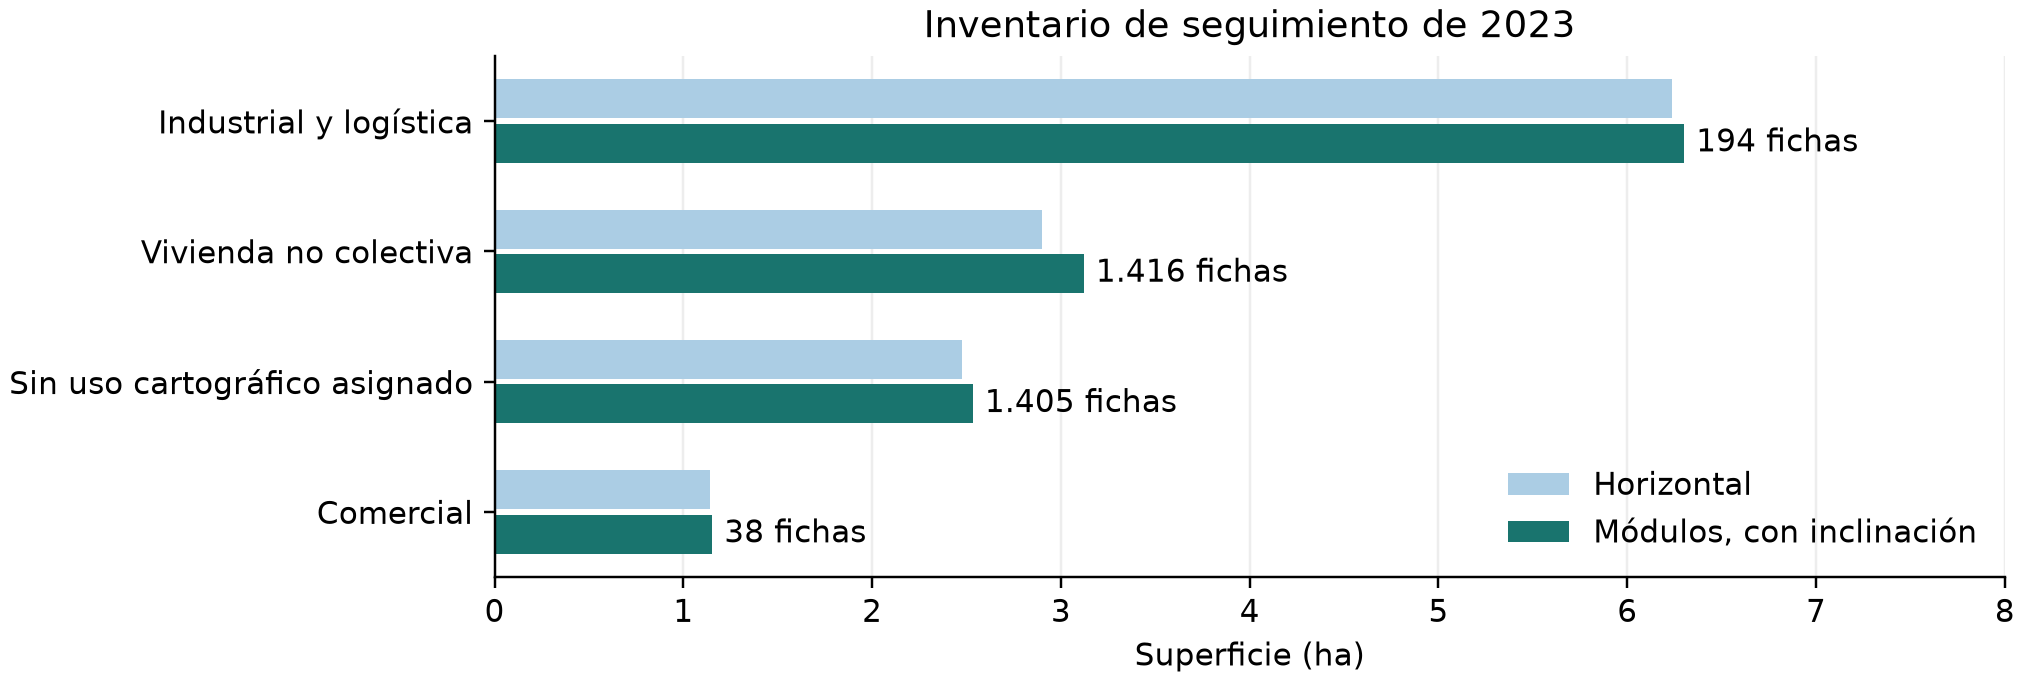
\includegraphics[width=\linewidth]{figuras/superficie_por_uso_2023.png}
\caption{Superficie horizontal y de módulos en cuatro categorías del inventario de seguimiento de 2023. Las etiquetas indican las fichas con paneles.}
\label{fig:usos}
\end{figure}

La categoría industrial y logística aporta 6,23 ha horizontales en 194 fichas, el 41\,\% del área de seguimiento de 2023. La vivienda no colectiva aporta 2,90 ha en 1\,416 fichas. Para estimar el área de módulos se divide la proyección horizontal entre el coseno de la inclinación de cada detección.

\clearpage

\section{Superficie por campaña y evolución}

El \textbf{inventario por campaña} reúne la superficie de los paneles que se delimitaron en cada vuelo. El panel permite consultar los totales por municipio y abrir la ficha para ver en qué fechas se fotografió cada conjunto.

\begin{figure}[!ht]
\centering
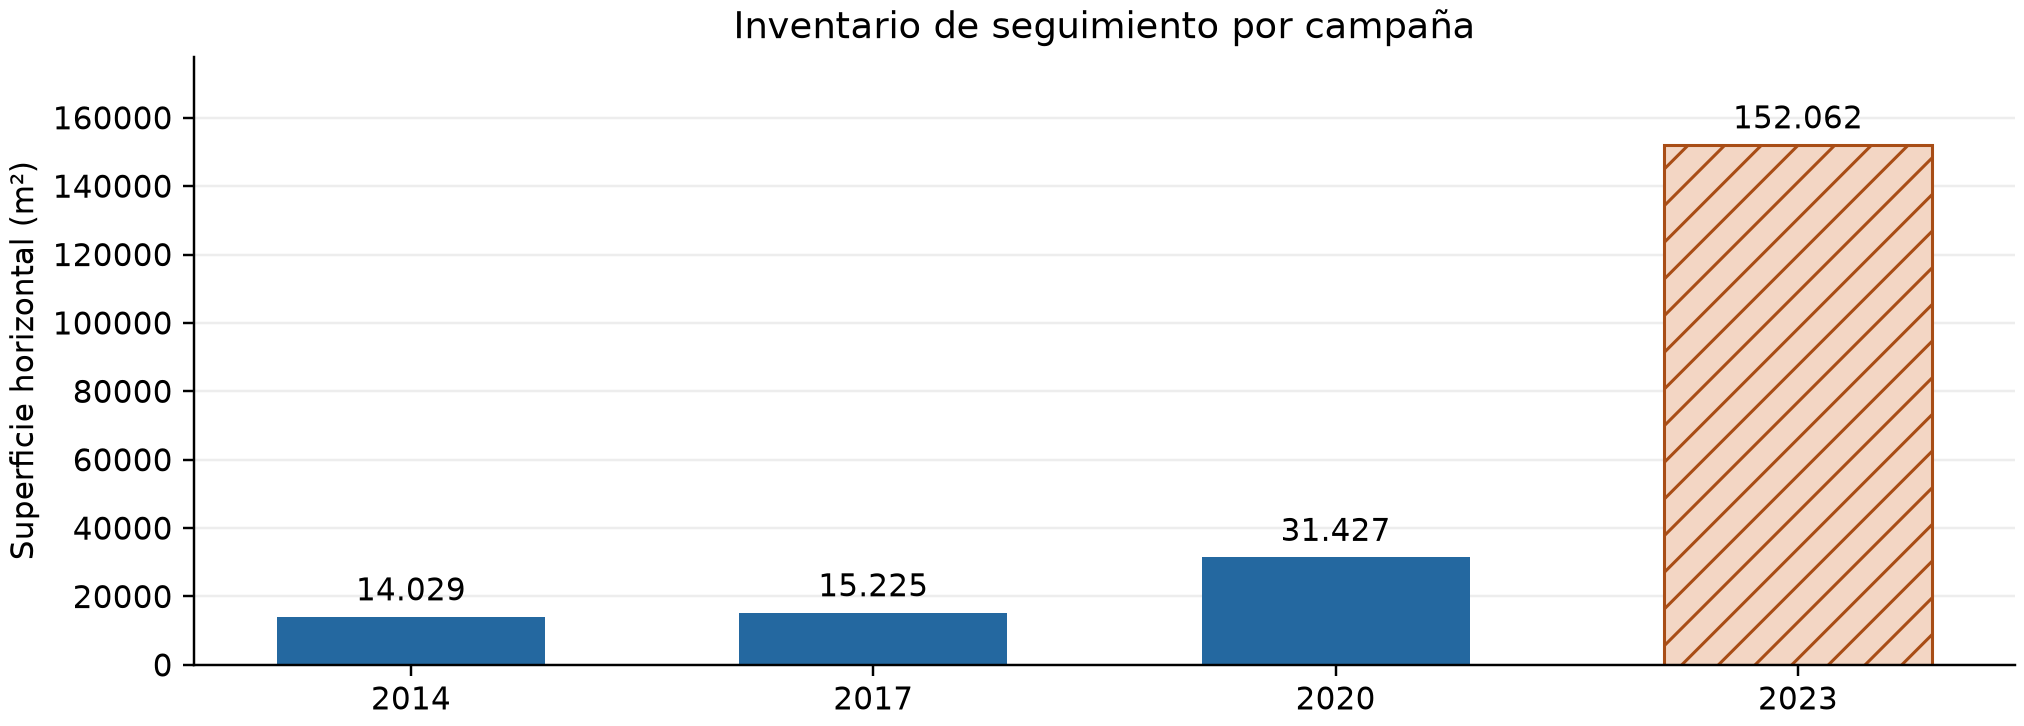
\includegraphics[width=\linewidth]{figuras/superficie_por_campania.png}
\caption{Superficie horizontal del inventario de seguimiento en cada vuelo. La barra rayada corresponde a las 15,21 ha de contornos automáticos de 2023 seleccionados para el seguimiento.}
\label{fig:historia}
\end{figure}

En el seguimiento se registraron \textbf{14\,029 m\textsuperscript{2} en 2014, 15\,225 en 2017, 31\,427 en 2020 y 152\,062 en 2023}. Los tres primeros totales se midieron sobre dibujos manuales en los encuadres revisados de cada vuelo. El último suma las máscaras automáticas seleccionadas para el seguimiento. Cada total refleja el alcance y la fuente de las observaciones de ese año.

La pestaña \textbf{Instalaciones y evolución} permite seleccionar un intervalo y localizar los emplazamientos donde cambia la superficie. Cuando se dispone de una ausencia revisada y de una primera presencia, la aparición queda acotada entre las fechas de los dos vuelos.

\clearpage

\section{Geometría de los paneles a partir de LiDAR}

El inventario de seguimiento contiene 8\,671 polígonos de 2023, con 15,21 ha de superficie horizontal. El ajuste aceptó una inclinación para 3\,973 polígonos (45,8\,\%) y una orientación para 3\,280 (37,8\,\%). En 693 se aceptó la pendiente, pero el cálculo energético conservó una orientación supuesta porque la inclinación era inferior a \(5^\circ\).

\begin{figure}[!ht]
\centering
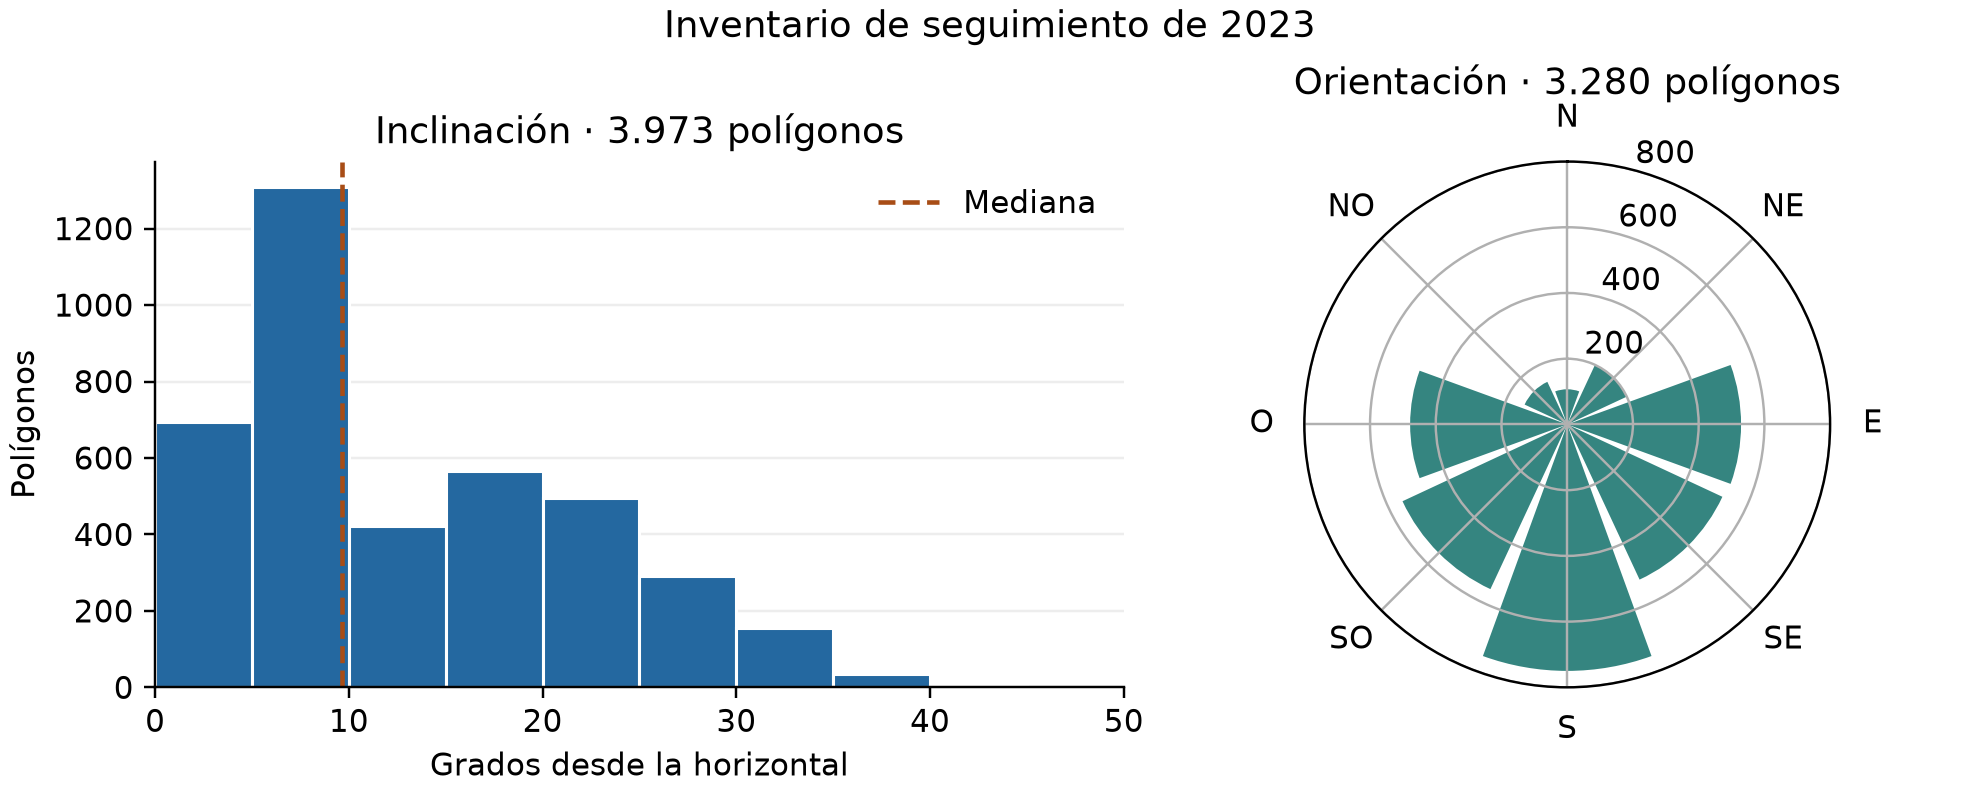
\includegraphics[width=\linewidth]{figuras/angulos_lidar_2023.png}
\caption{Ángulos aceptados en el inventario de seguimiento de 2023. Izquierda, inclinaciones en intervalos de \(5^\circ\). Derecha, orientaciones geográficas en ocho sectores de \(45^\circ\). Cada polígono cuenta una vez.}
\label{fig:angulos}
\end{figure}

Las pendientes aceptadas tienen una media de \textbf{\(13,0^\circ\)} y una mediana de \textbf{\(9,7^\circ\)}. Tres cuartas partes están por debajo de \(20^\circ\). El sector sur es el más frecuente (750 polígonos), con presencia también hacia el este y el oeste. Por superficie, la inclinación LiDAR se aplica al 59,6\,\% del área horizontal utilizada para calcular la energía de 2023.

Los ángulos aceptados se conservan. Si falta la inclinación se toma la mediana de las pendientes aceptadas del mismo uso del edificio, siempre que haya al menos 20 mediciones. Para los demás casos se usa la mediana general. La orientación al sur se usa como referencia cuando falta un azimut fiable. El origen de los valores se conserva en el CSV.

\clearpage

\section{Producción estimada y estacionalidad}

Las 15,21 ha horizontales del inventario de seguimiento de 2023 equivalen a 15,66 ha estimadas de módulos tras corregir la inclinación. La potencia nominal estimada es de 32,51 MWp. Para obtenerla se usa la eficiencia de referencia correspondiente al año atribuido a cada emplazamiento. Cuando el intervalo de aparición está acotado, se toma su punto medio. En el 57,4\,\% de la superficie, la primera evidencia disponible se utiliza como referencia de edad.

La producción de referencia es de \textbf{35,76 GWh/año} con el clima medio de PVGIS. La tabla muestra el efecto de cambiar solo las pérdidas operativas. La edad, la eficiencia de referencia y la geometría son las mismas en los tres cálculos. Se aplica aparte una degradación anual del 0,5\,\% según la edad.

\begin{table}[!ht]
\centering
\caption{Sensibilidad de la producción de 2023 a las pérdidas operativas.}
\label{tab:energia}
\begin{tabular}{lr}
\toprule
Pérdidas operativas & Producción estimada (GWh/año) \\
\midrule
12\,\% & 34,97 \\
10\,\% (referencia) & 35,76 \\
8\,\% & 36,56 \\
\bottomrule
\end{tabular}
\end{table}

\subsection{Producción mensual con la meteorología de 2023}

Las series cubren 3\,506 emplazamientos con paneles detectados en 2023. Su suma con pérdidas del 10\,\% da \textbf{36,19 GWh} al simular el inventario funcionando un año completo con la meteorología de 2023. La tabla~\ref{tab:energia} usa el clima medio de PVGIS.

\begin{figure}[!ht]
\centering
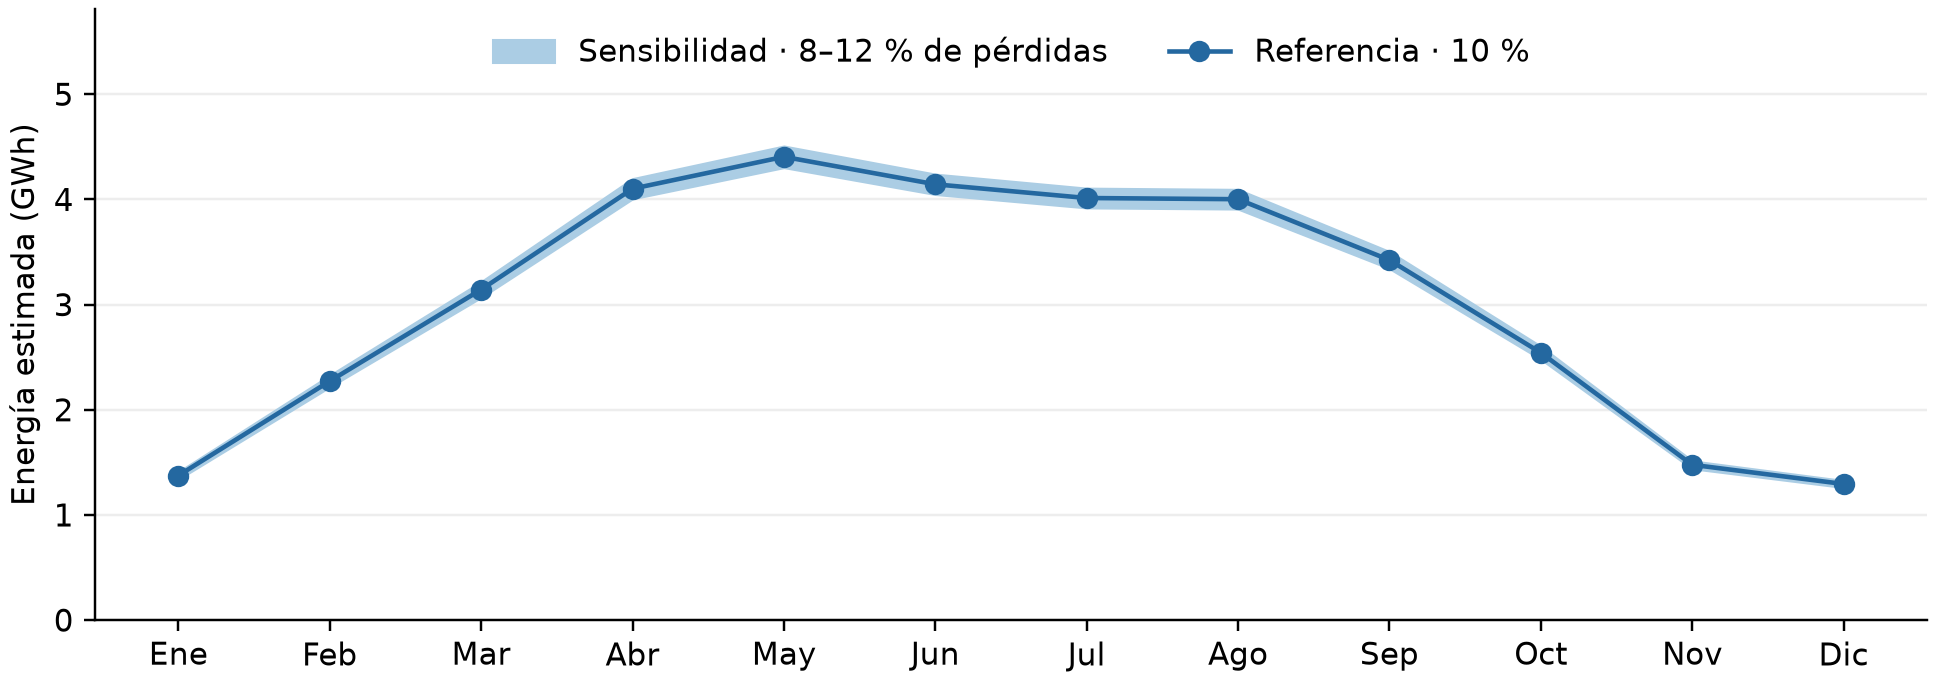
\includegraphics[width=\linewidth]{figuras/produccion_mensual_2023.png}
\caption{Producción mensual modelada en 2023. La línea usa el 10\,\% de pérdidas operativas y la banda abarca el 8--12\,\%.}
\label{fig:mensual}
\end{figure}

De mayo a agosto se concentra el 45,8\,\% de la energía de referencia. Mayo alcanza 4,41 GWh y diciembre 1,29 GWh.

\clearpage

\section{Distribución horaria de la producción}

La figura~\ref{fig:horas} compara cuatro geometrías con 1 kWp y la meteorología de 2023 en Santander. Al orientar los módulos hacia el sureste o el suroeste con \(30^\circ\) de inclinación, el pico medio de junio pasa de las 13:00 a las 16:00. Mirando al sur, pasar de \(10^\circ\) a \(30^\circ\) aumenta la producción de diciembre de 45,1 a 62,5 kWh por kWp. En junio, la referencia de \(10^\circ\) da 147,9 kWh y la de \(30^\circ\) da 142,3 kWh.

\begin{figure}[!ht]
\centering
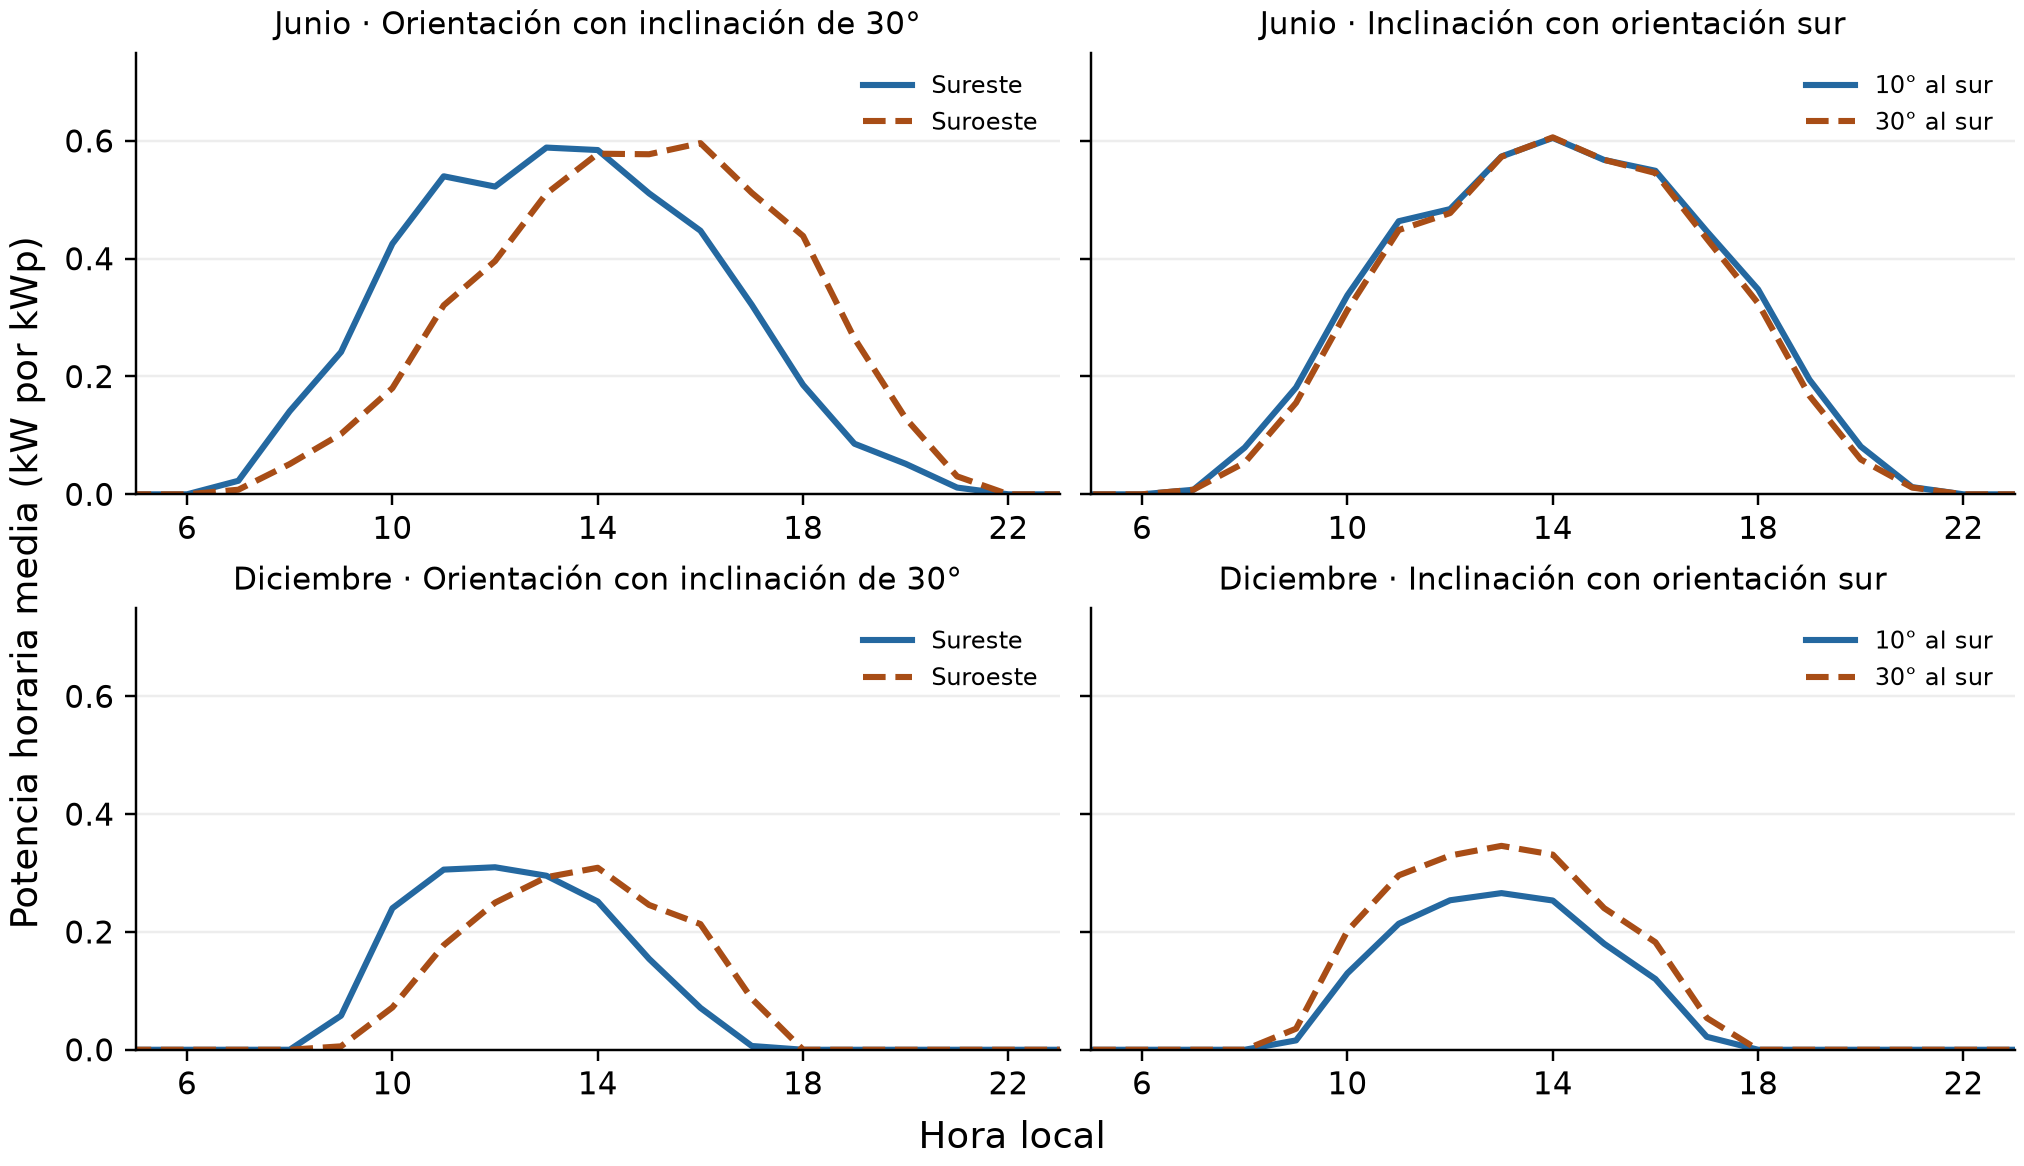
\includegraphics[width=\linewidth]{figuras/perfil_horario_santander_2023.png}
\caption{Potencia media por hora local de junio y diciembre de 2023. Referencias PVGIS por kWp, antes de aplicar pérdidas operativas y degradación.}
\label{fig:horas}
\end{figure}

\subsection*{De la curva de referencia a un tejado}

Como ejemplo, 100 m\textsuperscript{2} vistos desde arriba con \(30^\circ\) de inclinación equivalen a \(100/\cos(30^\circ)=115{,}5\) m\textsuperscript{2} de módulos. Con eficiencia de referencia del 17,7\,\% para 2017 se obtienen 20,44 kWp iniciales. Tras seis años de degradación y un 10\,\% de pérdidas, el factor que multiplica la curva es \(20{,}44 \times 0{,}995^6 \times 0{,}90\), aproximadamente 17,85. Con módulos de 2023 en la misma superficie y una eficiencia de referencia del 21,8\,\%, el factor es 22,66. A las 13:00 de un día medio de junio, la curva de \(30^\circ\) al sur da 0,573 kW por kWp. El resultado para esos dos tejados es de 10,2 kW y 13,0 kW, respectivamente.

\clearpage

\section{Aplicaciones de los resultados}

\subsection*{Actualizar un inventario de instalaciones}

Quien gestiona varios edificios puede cruzar sus ubicaciones con el mapa regional. Luego abre la ortofoto de los tejados con detección y comprueba cuáles ya tienen paneles. El resultado es una lista de edificios con su superficie visible y fecha de observación, útil para completar fichas o decidir dónde hacer una visita.

\subsection*{Comprobar si una obra figura en las imágenes}

Si una instalación figura como terminada antes de la fecha de la ortofoto, se puede localizar el tejado y revisar si los paneles eran visibles en ese vuelo. Si la imagen deja dudas, el caso pasa a revisión documental o a una visita. El mismo procedimiento sirve para seguir obras propias, contratadas o subvencionadas.

\subsection*{Elegir a qué hora usar la energía solar}

Un taller que puede mover la recarga de un vehículo compara la curva solar de su tejado con el consumo de sus equipos. Por ejemplo, si la recarga necesita 10 kWh y quedan disponibles 4 kWh solares en un horario y 8 en otro, el segundo aprovecharía 4 kWh solares más. La serie del proyecto aporta la generación estimada. La instalación necesita además su perfil de consumo para hacer la comparación.

\section{Dónde consultar las salidas}

{\small\raggedright
\begin{itemize}
\item \textbf{Panel interactivo.} Abrir \path{runs/visualizacion/panel_indicadores.html} en el navegador. El fondo de ortofoto requiere conexión. Para ver la ficha histórica de la nave de la figura~\ref{fig:pielagos}, seleccionar la campaña de 2020 y buscar \path{fv_832b218af089554de012} en \textbf{Instalaciones y evolución}.
\item \textbf{Mapas y figuras.} Las imágenes de este informe están en \path{docs/figuras/}. El mapa regional usa \path{municipios.gpkg} de \path{runs/indicadores/unet_actual/}. En la misma carpeta están \path{detecciones.gpkg} y el cruce con edificios. La tabla municipal del panel está en \path{runs/visualizacion/resumen_municipal.csv} y la geometría de seguimiento en \path{runs/indicadores/seguimiento_historico/atribucion.gpkg}.
\item \textbf{Evaluación del detector.} \path{runs/evaluacion/unet_actual/} contiene el resumen y los resultados por tesela. El protocolo se describe en la memoria técnica.
\item \textbf{Nubes LiDAR y planos.} El visor de resultados muestra ortofoto, nube 3D y superficies ajustadas por detección. El comando está en \path{docs/lidar/README.md}. Los motivos de aceptación o descarte se guardan en \path{runs/lidar/cantabria_20261112_v2/resumen.csv}; los ángulos utilizados para energía están en \path{runs/visualizacion/factores_energia.csv}.
\item \textbf{Producción con clima medio.} La tabla~\ref{tab:energia} usa \path{runs/visualizacion/produccion_estimada.csv}. \path{energia_paneles.csv} recoge superficies, potencia y energía por detección.
\item \textbf{Series con meteorología de 2023.} En \path{runs/visualizacion/series_temporales/inventario_2023_meteo_2023/} están los CSV mensuales, anuales y horarios. La curva de la nave de Piélagos está en \path{runs/visualizacion/consulta_pielagos/produccion.html}. La figura~\ref{fig:horas} usa el punto 34063939075 del índice de referencias PVGIS.
\end{itemize}
}

\end{document}
